\documentclass[autocontact]{gaceta}
\usepackage[utf8]{inputenc}

%---------------------
%-----librerias para los grafos
\usepackage{tikz}
\usetikzlibrary{positioning}
\definecolor {processblue}{cmyk}{0.96,0,0,0}

\usepackage{enumerate}
\usepackage{diagbox}
\usepackage{caption}
\captionsetup{justification=centerlast,labelfont=bf,textfont=it}
%---------------------
% Esto ya lo carga el estilo de La Gaceta:
\usepackage{amsmath, amsthm, amssymb}
%\usepackage{url} % <-- Para p\'aginas web o similar: \url{...}
\usepackage{graphicx}
%---------------------

%---------------------
% Carga esto para gr\'aficos si lo necesitas:
% \usepackage{wrapfig}
%---------------------

%---------------------
% <<< ESTO SE AJUSTAR\'A AL EDITAR CADA N\'UMERO DE LA GACETA >>>
\setcounter{page}{1} 
\journame{UAdeC-FCFM}
\yearofpublication{2018}
%\volume{1}
%\issuenumber{0}
%---------------------

%---------------------
% Deja esto as\'{\i}:
\belongstopart{Teoría de grafos} 


%---------------------
\title{Universidad Autónoma de Coahuila \\ Facultad de Ciencias Físico Matemáticas
\\ Investigación de operaciones \\ Teoría de Grafos \\ Tarea 2 \\ Alibeit Kakes}
\author{Jesús López Zavala} % o \author{Un Autor y Otro Autor}, etc.
% Opcional:
\shorttitle{Investigación de Operaciones}
%---------------------

%---------------------
\contact{Un autor, Dpto. de Matem\'aticas, Universidad de \dots}
{autor@uni.es}{http://www.uni.es/personales/autor.html}
%% SINTAXIS (\'usense tantos de estos como autores haya):
%\contact{nombre y direcci\'on autor 1}{email autor 1}{p\'agina web autor 1}
%\contact{nombre y direcci\'on autor 2}{email autor 2}{p\'agina web autor 2}
% (IMPORTANTE: se puede dejar vac\'{\i}o lo que se quiera)
%---------------------

%---------------------------
\begin{document}
\maketitle
%---------------------


%%---------------------------Problema1----------------------------------
%-----------------------------------------------------------------------
\section{Problema 1}
    Encontrar el camino de longitud máxima que une los nodos $x_{1}$ y $x_{6}$.
    
    \tikzstyle{camino}=[bottom color = processblue!20, draw,processblue, text = red]
    \tikzstyle{place}=[circle,draw=blue!50,fill=blue!20,thick]
    \tikzstyle{transition}=[rectangle,draw=black!50,fill=black!20,thick]
    \tikzstyle{every label}= [blue]
    
    \input{graphs/graphProblem1.tex}

    Para resolverlo hay que aplicar el algoritmo de Ford, a continuación se muestran los pasos 
    aplicados para generar cada una de las marcas:
    \begin{enumerate}
        \item Marcaremos el inicio del camino con la marca $(-,0).$
        \item Marcaremos cada uno de los nodos $j$  con una marca de la forma $(i, e(j))$, donde 
        $ e(j) = max \{e(i) + c(i,j)\}$ y $c(i, j)$ es la longitud del arco que conecta a $i$ y a $j$.
            Para iniciar tomaremos a $x_1$ como el nodo i; de forma que 
            las marcas que apareceran en los nodos $x_2$ y $x_3$ serán $(x_1, 1)$ y $(x_1, 2)$ 
            respectivamente.
        \item Para marcar el nodo $i = x_4$, los nodos $j = \{ x_1, x_2, x_3\}$ deberan esta marcados.
            Como en el paso anterior ésto ya se realizo, ahora podremos elegir entre el conjunto de marcas
            $e(j)$ la que es máxima, de ésta forma la marca que acompaña al nodo $x_4$ es $(x_2, 16)$.
        \item Para marcar $x_4$ aplicamos el mismo razonamiento que en el paso anterior y el resultado
        de la marca es: $(x_2, 32)$.
        \item Finalmente el nodo $x_6$ se quedará con la marca $(x_5, 36)$.
    \end{enumerate}
    A continuación se muestra el procedimiento hecho anteriormente para conseguir cada una de las 
    marcas. 
    \begin{figure}[h]

    \begin{tikzpicture}[-latex, auto, node distance =4 cm and 5cm, on grid , semithick, scale = 1.0,
            state/.style ={ circle ,top color =white , bottom color = processblue!20 ,
            draw,processblue , text=blue , minimum width =1 cm, scale = 1.0}]
        
        %\node [estilo del nodo] (nombre del nodo) [posicion relativa]/at (posicion,absoluta) {};
        \node[state] (n1) at (-5, 0) [label=left:$ (-{,}0) $] {$x_1$};
        \node[state] (n2) at (-2.5, 2.5) [label = above: $ (x_1 {,} 1) $] {$x_2$};
        \node[state] (n3) at (-2.5, -2.5) [label = above: $ (x_1 {,} 2) $] {$x_3$};
        \node[state] (n4) at (2.5, -2.5) [label = above: $ (x_2 {,} 16) $] {$x_4$};
        \node[state] (n5) at (2.5, 2.5) [label = above: $ (x_2 {,} 32) $] {$x_5$};
        \node[state] (n6) at (5, 0) [label = right: $ (x_5 {,} 36) $] {$x_6$};
        

        \path (n1)[camino] edge [bend right = -25] node[above = 0.15 cm] {$1$} (n2);
        \path (n1) edge [bend right = 25] node[below = 0.0 cm] {$2$} (n3);
        \path (n2)[camino] edge  node[above = 0.15 cm] {$31$} (n5);
        \path (n3) edge  node[above = 0.15 cm] {$12$} (n4);
        \path (n5)[camino] edge  [bend right = -25] node[above = 0.15 cm] {$4$} (n6);
        \path (n4) edge  [bend right = 25] node[below = 0.15 cm] {$2$} (n6);
        \path (n1) edge  node[above = 0.15 cm] {$30$} (n5);
        \path (n2) edge  [bend right = 25] node[above = 0.15 cm] {$15$} (n4);
        %si queremos un loop
        %\path (A) edge [loop left] node[left] {$1/4$} (A);
    \end{tikzpicture}

    \caption{Marcas realizadas en cada nodo, en azul se muestra el camino óptimo encontrado.}
\end{figure}

    Para encontrar el camino óptimo realizamos la siguiente operación:
    
    \begin{equation}\label{eq:p1-1}
        e(j) - e(i) = c(ij),
    \end{equation}
    
    y si esta ecuación se cumple entonces nos quedamos con el arco entre ambas marcas.
    Este análisis conduce al siguiente conjunto de arcos que conforman el camino de longitud máxima:
    
    \begin{equation}
        U = \{ (x_1, x_2), (x_2, x_5), (x_5, x_6) \}.    
    \end{equation}
    




%%---------------------------Problema2----------------------------------
%-----------------------------------------------------------------------

\section{Problema}
    ¿Podemos conocer la longitud del camino extremal sin conocer explícitamente los arcos que la 
    componen?. ¿Se pueden marcar más de una vez los vértices? \\
    \\Para conocer la longitud del camino extremal es necesario conocer explícitamente
        la relacion que existe entre los vértices (arcos), así como el valor que cada uno de los arcos tiene
        asignado. Si marcamos más de una vez los vértices, entonces no habrá ambiguedad y el algoritmo con el que
        se esté trabajando, para nuestro caso el algoritmo de Ford, encontrará todos las soluciones extremales del 
        problema dado. Esto es porque se pondran más de una marca en un nodo si la longitud medida al llegar a dicho
        nodo es igual para un determinado número de arcos.





%%---------------------------Problema3----------------------------------
%-----------------------------------------------------------------------
\section{Problema}
    Formule el algoritmo de Ford para hallar caminos mínimos.\\
    \\Supongamos que se quiere encontrar el camino mínimo entre los vértices $s$ y $t$ de algún grafo dado,
        para hacerlo formularemos el algoritmo de Ford como sigue:
        \begin{center}
            \begin{enumerate}
                \item Marcar el vértice $s$ con la marca $(-, 0)$.
                \item Marcar el vértice $j$ con la marca $(i, e(j))$, con 
                    \begin{equation}\label{eq:p2-1}
                        e(j) = min \{e(i) + c(i,j)\}. 
                    \end{equation}
                \item Aplicar el paso anterior hasta llegar al vértice $t$.
                \item Para encontrar el camino mínimo se hace un recorrido desde el vértice $t$ hasta el 
                        vértice $s$ buscando los arcos tales que cumplan: 
                        \begin{equation}\label{eq:p2-2}
                            e(j) - e(i) = c(i,j),
                        \end{equation}
                        de forma que el conjunto de arcos encontrados es el camino mínimo.
            \end{enumerate}
        \end{center}





%%---------------------------Problema4----------------------------------
%-----------------------------------------------------------------------
\section{Problema}
    En el grafo del ejercicio 1, halle el camino de longitud mínima.\\
    \\A continuación se muestran las marcas obtenidas al aplicar el algoritmo de Ford 
    descrito anteriormente:
    
       
    \begin{tikzpicture}[-latex, auto, node distance =4 cm and 5cm, on grid , semithick, scale = 1.0,
        state/.style ={ circle ,top color =white , bottom color = processblue!20 ,
        draw,processblue , text=blue , minimum width =1 cm, scale = 1.0}]
    
        %\node [estilo del nodo] (nombre del nodo) [posicion relativa]/at (posicion,absoluta) {};
        \node[state] (n1) at (-5, 0) [label=left:$ (-{,}0) $] {$x_1$};
        \node[state] (n2) at (-2.5, 2.5) [label = above: $ (x_1 {,} 1) $] {$x_2$};
        \node[state] (n3) at (-2.5, -2.5) [label = above: $ (x_1 {,} 2) $] {$x_3$};
        \node[state] (n4) at (2.5, -2.5) [label = above: $ (x_3 {,} 14) $] {$x_4$};
        \node[state] (n5) at (2.5, 2.5) [label = above: $ (x_1 {,} 30) $] {$x_5$};
        \node[state] (n6) at (5, 0) [label = right: $ (x_4 {,} 16) $] {$x_6$};
        

        \path (n1) edge [bend right = -25] node[above = 0.15 cm] {$1$} (n2);
        \path (n1)[camino] edge [bend right = 25] node[below = 0.0 cm] {$2$} (n3);
        \path (n2) edge  node[above = 0.15 cm] {$31$} (n5);
        \path (n3)[camino] edge  node[above = 0.15 cm] {$12$} (n4);
        \path (n5) edge  [bend right = -25] node[above = 0.15 cm] {$4$} (n6);
        \path (n4)[camino] edge  [bend right = 25] node[below = 0.15 cm] {$2$} (n6);
        \path (n1) edge  node[above = 0.15 cm] {$30$} (n5);
        \path (n2) edge  [bend right = 25] node[above = 0.15 cm] {$15$} (n4);
        %si queremos un loop
        %\path (A) edge [loop left] node[left] {$1/4$} (A);
    \end{tikzpicture}

    
    \pagebreak
    Aplicando la ecuación \eqref{eq:p2-2}, la cual fue descrita en el paso $4$ del problema anterior, obtenemos el siguente conjunto de arcos:
    \begin{equation}\label{eq:p4-1}
        U = \{ (x_1, x_3), (x_3, x_4), (x_4, x_6)\},    
    \end{equation}
    %$$ U = \{ (x_1, x_3), (x_3, x_4), (x_4, x_6)\}, $$
    siendo éste el camino de longitud \eqref{eq:p4-1} mínima.
    


%%---------------------------Problema5----------------------------------
%-----------------------------------------------------------------------
\section{Problema}
    En el grafo siguiente halle:
    
    \begin{center}
        \begin{enumerate}[a)]
            \item Encontrar el camino de longitud máxima que une los nodos $\alpha$ y $\beta$.
            \item Encontrar el camino de longitud mínima que une los nodos $\alpha$ y $\beta$.
            \item El recorrido que acumule la menor cantidad de arcos, de $\alpha$ a $\beta$.
        \end{enumerate}
    \end{center}
    
    \begin{figure}[h]
    
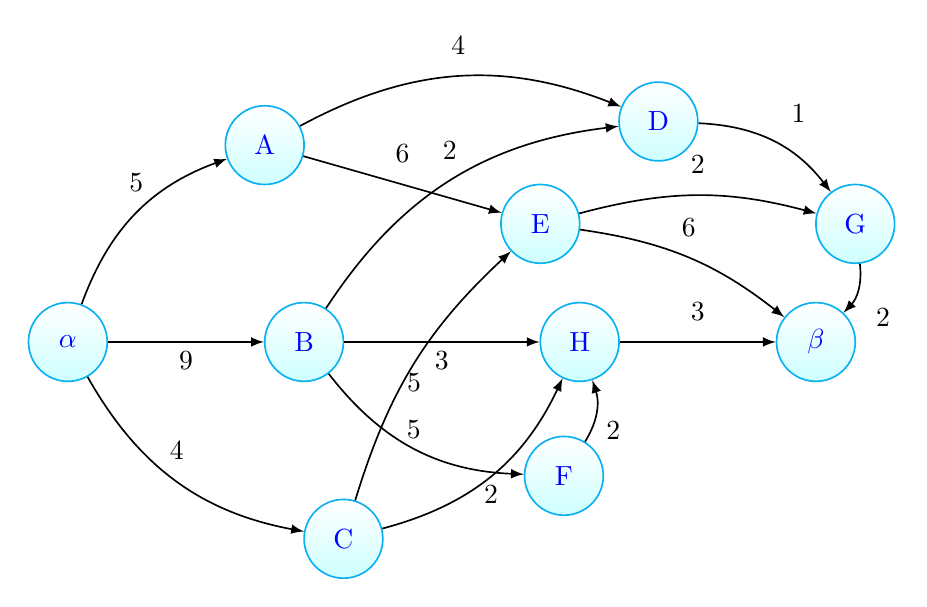
\begin{tikzpicture}[-latex, auto, node distance =4 cm and 5cm, on grid , semithick, scale = 1.0,
            state/.style ={ circle ,top color =white , bottom color = processblue!20 ,
            draw,processblue , text=blue , minimum width =1 cm, scale = 1.0}]
        
        %\node [estilo del nodo] (nombre del nodo) [posicion relativa]/at (posicion,absoluta) {};
        \node[state] (a) at (-5, 0) {$\alpha$};
        \node[state] (A) at (-2.5, 2.5) {A};
        \node[state] (B) at (-2.0, 0) {B};
        \node[state] (C) at (-1.5, -2.5) {C};
        \node[state] (E) at (1.0, 1.5) {E};
        \node[state] (H) at (1.5, 0) {H};
        \node[state] (F) at (1.3, -1.7) {F};
        \node[state] (D) at (2.5, 2.8) {D};
        \node[state] (b) at (4.5, 0) {$\beta$};
        \node[state] (G) at (5.0, 1.5) {G};
        

        \path (a) edge [bend right = -25] node[above = 0.15 cm] {$5$} (A);
        \path (a) edge node[below = 0.0 cm] {$9$} (B);
        \path (a) edge [bend right = 25] node[above = 0.15 cm] {$4$} (C);
        \path (A) edge [bend right = -25] node[above = 0.15 cm] {$4$} (D);
        \path (A) edge node[above = 0.15 cm] {$6$} (E);
        \path (B) edge  [bend right = -25] node[above = 0.15 cm] {$2$} (D);
        \path (B) edge  node[below = 0.0 cm] {$3$} (H);
        \path (B) edge  [bend right = 25] node[above = 0.0 cm] {$5$} (F);
        \path (C) edge [bend right = -15] node[below = 0.0 cm] {$5$} (E);
        \path (C) edge [bend right = 25] node[below = 0.0 cm] {$2$} (H);
        \path (F) edge [bend right = 25] node[below right = 0.0 cm] {$2$} (H);
        \path (H) edge node[above = 0.15 cm] {$3$} (b);
        \path (G) edge [bend right = -25] node[below right = 0.15 cm] {$2$} (b);
        \path (D) edge [bend right = -25] node[above right = 0.15 cm] {$1$} (G);
        \path (E) edge [bend right = -15] node[above = 0.15 cm] {$2$} (G);
        \path (E) edge [bend right = -15] node[above = 0.15 cm] {$6$} (b);
        
        %si queremos un loop
        %\path (A) edge [loop left] node[left] {$1/4$} (A);
    \end{tikzpicture}


    \caption{}
\end{figure}
    \pagebreak
    a) Aplicando el algoritmo de Ford se obtiene que el conjunto:
    \begin{equation}
        U = \{ (\alpha, B), (B, F), (F, H), (H, \beta) \},     
    \end{equation}
    
    es el camino de longitud máxima. En la figura se puede observar a este conjunto de arcos 
    coloreados en tono azul:

    \begin{figure}[h]


\begin{tikzpicture}[-latex, auto, node distance =4 cm and 5cm, on grid , semithick, scale = 1.0,
        state/.style ={ circle ,top color =white , bottom color = processblue!20 ,
        draw,processblue , text=blue , minimum width =1 cm, scale = 1.0}]
    
    %\node [estilo del nodo] (nombre del nodo) [posicion relativa]/at (posicion,absoluta) {};
    \node[state] (a) at (-5, 0) [label = left: $ (- {,} 0) $] {$\alpha$};
    \node[state] (A) at (-2.5, 2.5) [label = above: $ (\alpha {,} 5) $] {A};
    \node[state] (B) at (-2.0, 0) [label = above left: $ (\alpha {,} 9) $] {B};
    \node[state] (C) at (-1.5, -2.5) [label = above left: $ (\alpha {,} 4) $] {C};
    \node[state] (E) at (1.0, 1.5) [label = above: $ (A {,} 11) $] {E};
    \node[state] (H) at (1.5, 0) [label = above: $ (F {,} 16) $] {H};
    \node[state] (F) at (1.3, -1.7) [label = below: $ (B {,} 14) $] {F};
    \node[state] (D) at (2.5, 2.8) [label = above: $ (B {,} 11) $] {D};
    \node[state] (b) at (4.5, 0) [label = above: $ (H {,} 19) $] {$\beta$};
    \node[state] (G) at (5.0, 1.5) [label = above: $ (E {,} 13) $] {G};
    

    \path (a) edge [bend right = -25] node[above = 0.15 cm] {$5$} (A);
    \path (a)[camino] edge node[below = 0.0 cm] {$9$} (B);
    \path (a) edge [bend right = 25] node[above = 0.15 cm] {$4$} (C);
    \path (A) edge [bend right = -25] node[above = 0.15 cm] {$4$} (D);
    \path (A) edge node[above = 0.15 cm] {$6$} (E);
    \path (B) edge  [bend right = -25] node[above = 0.15 cm] {$2$} (D);
    \path (B) edge  node[below = 0.0 cm] {$3$} (H);
    \path (B)[camino] edge  [bend right = 25] node[above = 0.0 cm] {$5$} (F);
    \path (C) edge [bend right = -15] node[below = 0.0 cm] {$5$} (E);
    \path (C) edge [bend right = 25] node[below = 0.0 cm] {$2$} (H);
    \path (F)[camino] edge [bend right = 25] node[below right = 0.0 cm] {$2$} (H);
    \path (H)[camino] edge node[above = 0.15 cm] {$3$} (b);
    \path (G) edge [bend right = -25] node[below right = 0.15 cm] {$2$} (b);
    \path (D) edge [bend right = -25] node[above right = 0.15 cm] {$1$} (G);
    \path (E) edge [bend right = -15] node[above = 0.15 cm] {$2$} (G);
    \path (E) edge [bend right = -15] node[above = 0.15 cm] {$6$} (b);


    %si queremos un loop
    %\path (A) edge [loop left] node[left] {$1/4$} (A);
    \end{tikzpicture}

    \caption{Camino de longitud máxima entre los nodos $\alpha$ y $\beta$.}
\end{figure}


    b) El algoritmo de Ford para encontrar caminos mínimos conduce a que el siguiente conjunto:
    \begin{equation}
        U = \{ (\alpha, C), (C, H), (H, \beta) \},
    \end{equation}
    
    es el camino de longitud mínima.\\ A continuación se muestra la figura con las marcas resultantes 
    en cada vértice, así como los arcos que conforman 
    al conjunto $U$. Dichos arcos estan coloreados en azul y sus respectivas longitudes se muestran en 
    color rojo:

    \begin{figure}[h]

\begin{tikzpicture}[-latex, auto, node distance =4 cm and 5cm, on grid , semithick, scale = 1.0,
        state/.style ={ circle ,top color =white , bottom color = processblue!20 ,
        draw,processblue , text=blue , minimum width =1 cm, scale = 1.0}]
    
    %\node [estilo del nodo] (nombre del nodo) [posicion relativa]/at (posicion,absoluta) {};
    \node[state] (a) at (-5, 0) [label = left: $ (- {,} 0) $] {$\alpha$};
    \node[state] (A) at (-2.5, 2.5) [label = above: $ (\alpha {,} 5) $] {A};
    \node[state] (B) at (-2.0, 0) [label = above left: $ (\alpha {,} 9) $] {B};
    \node[state] (C) at (-1.5, -2.5) [label = above left: $ (\alpha {,} 4) $] {C};
    \node[state] (E) at (1.0, 1.5) [label = above: $ (C {,} 9) $] {E};
    \node[state] (H) at (1.5, 0) [label = above: $ (C {,} 6) $] {H};
    \node[state] (F) at (1.3, -1.7) [label = below: $ (B {,} 14) $] {F};
    \node[state] (D) at (2.5, 2.8) [label = above: $ (A {,} 9) $] {D};
    \node[state] (b) at (4.5, 0) [label = above: $ (H {,} 9) $] {$\beta$};
    \node[state] (G) at (5.0, 1.5) [label = above: $ (D {,} 10) $] {G};
    

    \path (a) edge [bend right = -25] node[above = 0.15 cm] {$5$} (A);
    \path (a) edge node[below = 0.0 cm] {$9$} (B);
    \path (a)[camino] edge [bend right = 25] node[above = 0.15 cm] {$4$} (C);
    \path (A) edge [bend right = -25] node[above = 0.15 cm] {$4$} (D);
    \path (A) edge node[above = 0.15 cm] {$6$} (E);
    \path (B) edge  [bend right = -25] node[above = 0.15 cm] {$2$} (D);
    \path (B) edge  node[below = 0.0 cm] {$3$} (H);
    \path (B) edge  [bend right = 25] node[above = 0.0 cm] {$5$} (F);
    \path (C) edge [bend right = -15] node[below = 0.0 cm] {$5$} (E);
    \path (C)[camino] edge [bend right = 25] node[below = 0.0 cm] {$2$} (H);
    \path (F) edge [bend right = 25] node[below right = 0.0 cm] {$2$} (H);
    \path (H)[camino] edge node[above = 0.15 cm] {$3$} (b);
    \path (G) edge [bend right = -25] node[below right = 0.15 cm] {$2$} (b);
    \path (D) edge [bend right = -25] node[above right = 0.15 cm] {$1$} (G);
    \path (E) edge [bend right = -15] node[above = 0.15 cm] {$2$} (G);
    \path (E) edge [bend right = -15] node[above = 0.15 cm] {$6$} (b);


    %si queremos un loop
    %\path (A) edge [loop left] node[left] {$1/4$} (A);
    \end{tikzpicture}

    \caption{}
\end{figure}

    c) Para responder a esta pregunta, sustituiremos los valores predeterminados en cada 
    arco por el valor de 1, luego aplicaremos el algoritmo de Ford para encontrar así 
    todos los posibles conjuntos con el menor número de arcos.
    \\Luego de aplicar el algoritmo, el grafo reslultante se muestra a continuación:

    \pagebreak

        \begin{tikzpicture}[-latex, auto, node distance =4 cm and 5cm, on grid , semithick, scale = 1.0,
        state/.style ={ circle ,top color =white , bottom color = processblue!20 ,
        draw,processblue , text=blue , minimum width =1 cm, scale = 1.0}]
    
        %\node [estilo del nodo] (nombre del nodo) [posicion relativa]/at (posicion,absoluta) {};
        \node[state] (a) at (-5, 0) [label = left: $ (- {,} 0) $] {$\alpha$};
        \node[state] (A) at (-2.5, 2.5) [label = above: $ (\alpha {,} 1) $] {A};
        \node[state] (B) at (-2.0, 0) [label = above left: $ (\alpha {,} 1) $] {B};
        \node[state] (C) at (-1.5, -2.5) [label = above left: $ (\alpha {,} 1) $] {C};
        \node[state] (E) at (1.0, 1.5) [label = above: $ (A {,} 2) $] [label = above right: $ (C {,} 2) $] {E};
        \node[state] (H) at (1.5, 0) [label = above: $ (F {,} 3) $] {H};
        \node[state] (F) at (1.3, -1.7) [label = below: $ (B {,} 2) $] {F};
        \node[state] (D) at (2.5, 2.8) [label = above: $ (A {,} 2) $] [label = above right: $ (B {,} 2) $] {D};
        \node[state] (b) at (4.5, 0) [label = below left: $ (H {,} 4) $] [label = below: $ (G {,} 4) $] {$\beta$};
        \node[state] (G) at (5.0, 1.5) [label = above: $ (D {,} 3) $] [label = above right: $ (E {,} 3) $] {G};
        

        \path (a) edge [bend right = -25] node[above = 0.15 cm] {$1$} (A);
        \path (a)[camino] edge node[below = 0.0 cm] {$1$} (B);
        \path (a)[camino] edge [bend right = 25] node[above = 0.15 cm] {$1$} (C);
        \path (A) edge [bend right = -25] node[above = 0.15 cm] {$1$} (D);
        \path (A) edge node[above = 0.15 cm] {$1$} (E);
        \path (B) edge  [bend right = -25] node[above = 0.15 cm] {$1$} (D);
        \path (B) edge  node[below = 0.0 cm] {$1$} (H);
        \path (B)[camino] edge  [bend right = 25] node[above = 0.0 cm] {$1$} (F);
        \path (C) edge [bend right = -15] node[below = 0.0 cm] {$1$} (E);
        \path (C) edge [bend right = 25] node[below = 0.0 cm] {$1$} (H);
        \path (F)[camino] edge [bend right = 25] node[below right = 0.0 cm] {$1$} (H);
        \path (H)[camino] edge node[above = 0.15 cm] {$1$} (b);
        \path (G)[camino] edge [bend right = -25] node[below right = 0.15 cm] {$1$} (b);
        \path (D) edge [bend right = -25] node[above right = 0.15 cm] {$1$} (G);
        \path (E) edge [bend right = -15] node[above = 0.15 cm] {$1$} (G);
        \path (E) edge [bend right = -15] node[above = 0.15 cm] {$1$} (b);


        %si queremos un loop
        %\path (A) edge [loop left] node[left] {$1/4$} (A);
    \end{tikzpicture}

    Observamos que algunos vértices tienen asignadas más de una marca, ésto se hizo con el fin de 
    encontrar todas las soluciones al problema; las cuales son:
    \begin{center}
       \begin{equation}
            U_1 = \{(\alpha,A), (A,E), (E,\beta)\},              
       \end{equation}
       
       \begin{equation}
            U_2 = \{(\alpha,B), (B,H), (H,\beta)\},
       \end{equation}

       \begin{equation}
            U_3 = \{(\alpha,C), (C,E), (E,\beta)\},
       \end{equation}

       \begin{equation}
            U_4 = \{(\alpha,C), (C,H), (H,\beta)\},
       \end{equation}

       \begin{equation}
            U_5 = \{(\alpha,C), (C,E), (E,G), (G,\beta)\},
       \end{equation}

       \begin{equation}
            U_4 = \{(\alpha,A), (A,E), (E,G), (G,\beta)\}.
       \end{equation}
    \end{center}
    


%%---------------------------Problema6----------------------------------
%-----------------------------------------------------------------------
\section{Problema}
    El grafo sigueinte representa la estructura gerárgica de una organización, el nodo 
    $j$ es subordinado de $i$, si $j$ desciende de $i$ y si existe el arco $(i,j),$ entonces
    $j$ es subordinado directo de $i$.
    
    \begin{center}
        \begin{enumerate}[a)]
            \item ¿Cuáles y cuantos subordinados directos tine cada elemento del sistema?
            \item ¿Cuál es el total de subordinados de los vértices $1$ y $9$?
            \item Halle el camino de mayor clase de subordinación.
        \end{enumerate}        
    \end{center}

        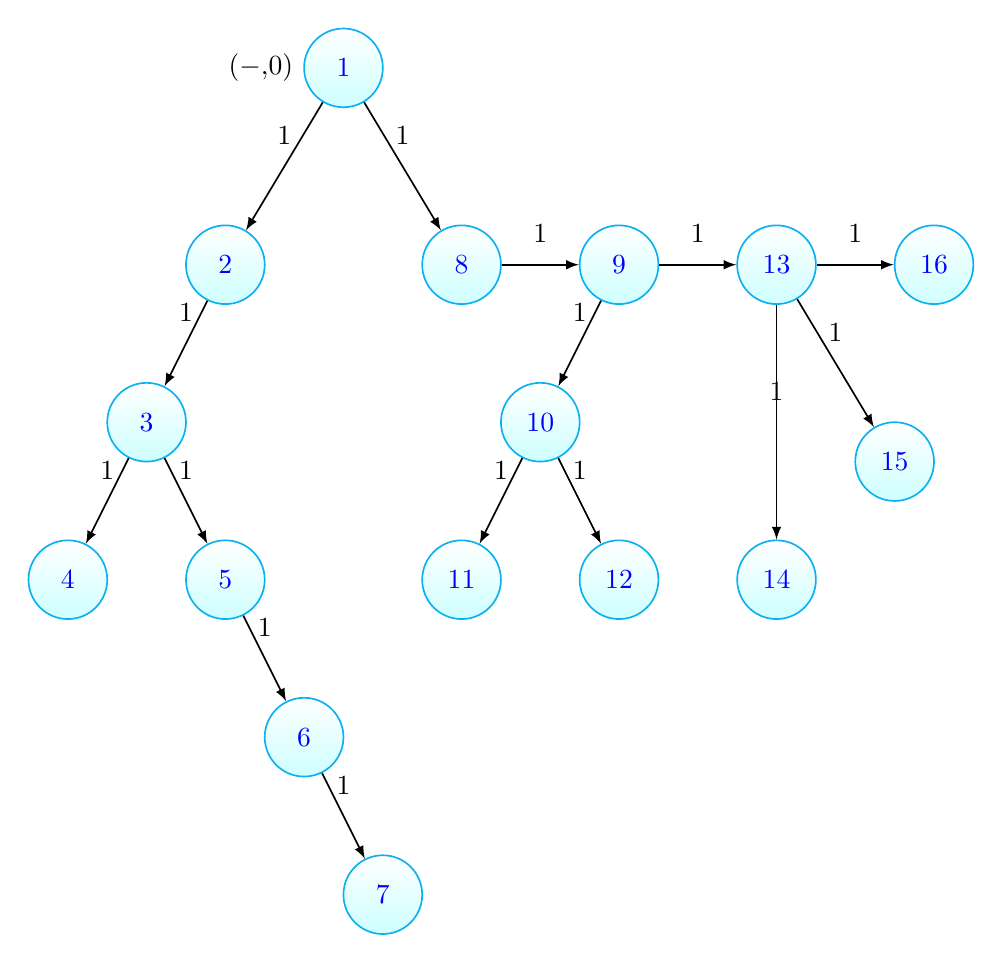
\begin{tikzpicture}[-latex, auto, node distance =4 cm and 5cm, on grid , semithick, scale = 1.0,
        state/.style ={ circle ,top color =white , bottom color = processblue!20 ,
        draw,processblue , text=blue , minimum width =1 cm, scale = 1.0}]
    
        %\node [estilo del nodo] (nombre del nodo) [posicion relativa]/at (posicion,absoluta) {};
        \node[state] (n1) at (0, 0) [label = left: $ (- {,} 0) $] {1};
        \node[state] (n2) at (-1.5, -2.5) {2};
        \node[state] (n3) at (-2.5, -4.5) {3};
        \node[state] (n4) at (-3.5, -6.5) {4};
        \node[state] (n5) at (-1.5, -6.5) {5};
        \node[state] (n6) at (-0.5, -8.5) {6};
        \node[state] (n7) at (0.5, -10.5) {7};
        \node[state] (n8) at (1.5, -2.5) {8};
        \node[state] (n9) at (3.5, -2.5) {9};
        \node[state] (n10) at (2.5, -4.5) {10};
        \node[state] (n11) at (1.5, -6.5) {11};
        \node[state] (n12) at (3.5, -6.5) {12};
        \node[state] (n13) at (5.5, -2.5) {13};
        \node[state] (n14) at (5.5, -6.5) {14};
        \node[state] (n15) at (7.0, -5.0) {15};
        \node[state] (n16) at (7.5, -2.5) {16};
        

        
        \path (n1) edge node[above = 0.15 cm] {$1$} (n2);
        \path (n1) edge node[above = 0.15 cm] {$1$} (n8);
        \path (n2) edge node[above = 0.15 cm] {$1$} (n3);
        \path (n3) edge node[above = 0.15 cm] {$1$} (n4);
        \path (n3) edge node[above = 0.15 cm] {$1$} (n5);
        \path (n5) edge node[above = 0.15 cm] {$1$} (n6);
        \path (n6) edge node[above = 0.15 cm] {$1$} (n7);
        
        \path (n8) edge node[above = 0.15 cm] {$1$} (n9);
        \path (n9) edge node[above = 0.15 cm] {$1$} (n10);
        \path (n10) edge node[above = 0.15 cm] {$1$} (n11);
        \path (n10) edge node[above = 0.15 cm] {$1$} (n12);

        \path (n9) edge node[above = 0.15 cm] {$1$} (n13);

        \path (n13) edge node[above = 0.15 cm] {$1$} (n14);
        \path (n13) edge node[above = 0.15 cm] {$1$} (n15);
        \path (n13) edge node[above = 0.15 cm] {$1$} (n16);
        
        %si queremos un loop
        %\path (A) edge [loop left] node[left] {$1/4$} (A);
    \end{tikzpicture}


    \pagebreak

    a) Se escribiran los elementos del sistema con sus respectivos subordinados directos.
    La notación $1,2,3,4\{2,5\}$, por ejemplo, significará que a los elementos 1, 2, 3 y 4 le corresponden 
    los elementos 2 y 5 como subordinados directos:

    \begin{center}
        \begin{enumerate}
            \item $4,7,11,12,14,15,16\{\phi \}.$
            \item $2\{3\}, 5\{6\}, 6\{7\},  8\{9\}.$
            \item $1\{2,8\},  3\{4,5\},   9\{10,13\}, 10\{11,12\}.$
            \item $13\{14,15,16\}.$
        \end{enumerate}
    \end{center}

    b) El vértice 1 tiene como subordinados un total de 14 elementos, mientras que el vértice 9 tiene
    tiene un total de 7 subordinados.

    c) Para responder a esta pregunta se le dio el valor de 1 a cada arco que se muestra en la Figura 8,
    luego se aplicó el algoritmo de Ford para encontrar el camino con mayor número de arcos, los 
    resultados obtenidos se muestran en la siguiente figura:

    \begin{figure}[h]


    \begin{tikzpicture}[-latex, auto, node distance =4 cm and 5cm, on grid , semithick, scale = 1.0,
            state/.style ={ circle ,top color =white , bottom color = processblue!20 ,
            draw,processblue , text=blue , minimum width =1 cm, scale = 1.0}]
        
            %\node [estilo del nodo] (nombre del nodo) [posicion relativa]/at (posicion,absoluta) {};
            \node[state] (n1) at (0, 0) [label = left: $ (- {,} 0) $] {1};
            \node[state] (n2) at (-1.5, -2.5) [label = left: $ (1 {,} 1) $] {2};
            \node[state] (n3) at (-2.5, -4.5) [label = left: $ (2 {,} 2) $] {3};
            \node[state] (n4) at (-3.5, -6.5) [label = left: $ (3 {,} 3) $] {4};
            \node[state] (n5) at (-1.5, -6.5) [label = right: $ (3 {,} 3) $] {5};
            \node[state] (n6) at (-0.5, -8.5) [label = right: $ (5 {,} 4) $]{6};
            \node[state] (n7) at (0.5, -10.5) [label = left: $ (6 {,} 5) $] {7};
            \node[state] (n8) at (1.5, -2.5) [label = left: $ (1 {,} 1) $] {8};
            \node[state] (n9) at (3.5, -2.5) [label = above: $ (8 {,} 2) $] {9};
            \node[state] (n10) at (2.5, -4.5) [label = left: $ (9 {,} 3) $] {10};
            \node[state] (n11) at (1.5, -6.5) [label = below: $ (10 {,} 4) $] {11};
            \node[state] (n12) at (3.5, -6.5) [label = below: $ (10 {,} 4) $] {12};
            \node[state] (n13) at (5.5, -2.5) [label = above: $ (9 {,} 3) $] {13};
            \node[state] (n14) at (5.5, -6.5) [label = below: $ (13 {,} 4) $] {14};
            \node[state] (n15) at (7.0, -5.0) [label = below: $ (13 {,} 4) $] {15};
            \node[state] (n16) at (7.5, -2.5) [label = below: $ (13 {,} 14) $] {16};
            
    
            
            \path (n1)[camino] edge node[above = 0.15 cm] {$1$} (n2);
            \path (n1) edge node[above = 0.15 cm] {$1$} (n8);
            \path (n2)[camino] edge node[above = 0.15 cm] {$1$} (n3);
            \path (n3) edge node[above = 0.15 cm] {$1$} (n4);
            \path (n3)[camino] edge node[above = 0.15 cm] {$1$} (n5);
            \path (n5)[camino] edge node[above = 0.15 cm] {$1$} (n6);
            \path (n6)[camino] edge node[above = 0.15 cm] {$1$} (n7);
            
            \path (n8) edge node[above = 0.15 cm] {$1$} (n9);
            \path (n9) edge node[above = 0.15 cm] {$1$} (n10);
            \path (n10) edge node[above = 0.15 cm] {$1$} (n11);
            \path (n10) edge node[above = 0.15 cm] {$1$} (n12);
    
            \path (n9) edge node[above = 0.15 cm] {$1$} (n13);
    
            \path (n13) edge node[right = 0.15 cm] {$1$} (n14);
            \path (n13) edge node[above = 0.15 cm] {$1$} (n15);
            \path (n13) edge node[above = 0.15 cm] {$1$} (n16);
            
            %si queremos un loop
            %\path (A) edge [loop left] node[left] {$1/4$} (A);
        \end{tikzpicture}
    
    
        \caption{En azul se representa el camino con mayor número de arcos.}
    \end{figure}
    \pagebreak
    El camino con mayor número de arcos es:
    \begin{center}
        \begin{equation}
            U = \{ (1,2), (2,3), (3,5), (5,6), (6,7) \}.
        \end{equation}        
    \end{center}

%%---------------------------Problema7----------------------------------
%-----------------------------------------------------------------------
\section{Problema}
    Dado el siguiente grafo considere que:
    \begin{center}
        \begin{enumerate}[a)]
            \item El valor sobre los arcos mide la distancia  entre los vértices. Halle el camino 
                de longitud mínima entre $1$ y $6$.
            \item Si no se considera orientación, ¿variaría la longitud del grafo de menor longitud
                que une dichos vértices?.
        \end{enumerate}        
    \end{center}

    \input{graphs/graphProblem7-1.tex}
    \pagebreak
    a) Aplicando el algoritmo de Ford:

    \begin{figure}[h]

    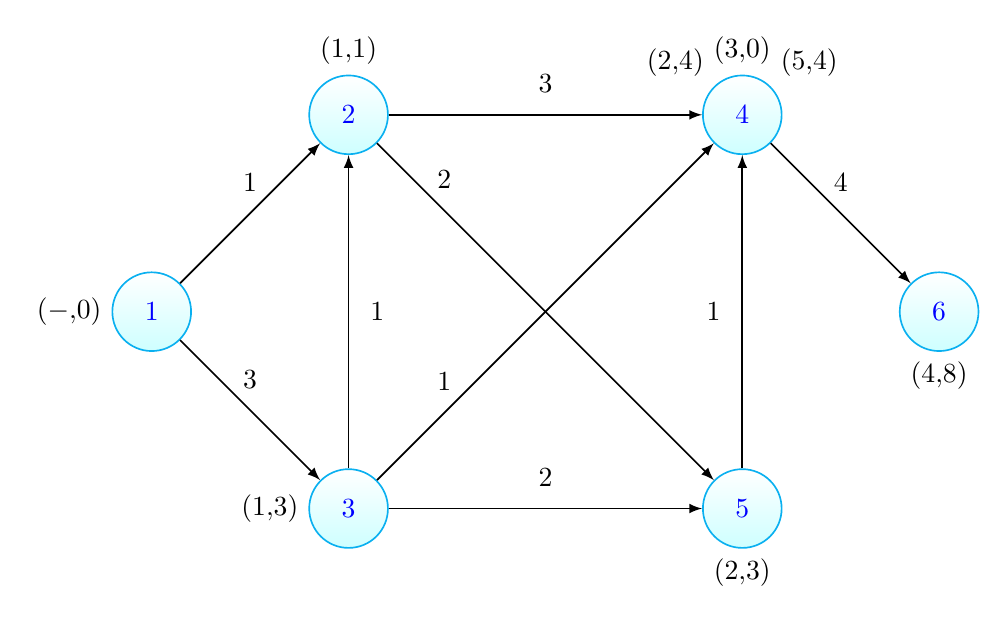
\begin{tikzpicture}[-latex, auto, node distance =4 cm and 5cm, on grid , semithick, scale = 1.0,
               state/.style ={ circle ,top color =white , bottom color = processblue!20 ,
               draw,processblue , text=blue , minimum width =1 cm, scale = 1.0}]
           
           %\node [estilo del nodo] (nombre del nodo) [posicion relativa]/at (posicion,absoluta) {};
           
           \node[state] (n1) at (-5, 0) [label = left: $ (- {,} 0) $] {1};
           \node[state] (n2) at (-2.5, 2.5) [label = above: $ (1 {,} 1) $] {2};
           \node[state] (n4) at (2.5, 2.5) [label = above left: $ (2 {,} 4) $] [label = above: $ (3 {,} 0) $] [label = above right: $ (5 {,} 4) $] {4};
           \node[state] (n6) at (5, 0) [label = below: $ (4 {,} 8) $] {6};
           \node[state] (n5) at (2.5, -2.5) [label = below: $ (2 {,} 3) $] {5};
           \node[state] (n3) at (-2.5, -2.5) [label = left: $ (1 {,} 3) $] {3};
           
           \path (n1) edge node[above = 0.15 cm] {$1$} (n2);
           \path (n1) edge node[above = 0.15 cm] {$3$} (n3);
   
           \path (n2) edge node[above = 0.15 cm] {$3$} (n4);
           \path (n2) edge node[above = 0.15 cm, pos = 0.20] {$2$} (n5);
   
           \path (n3) edge node[right = 0.15 cm] {$1$} (n2);
           \path (n3) edge node[above = 0.15 cm, pos = 0.20] {$1$} (n4);
           \path (n3) edge node[above = 0.15 cm] {$2$} (n5);
   
           \path (n5) edge node[left = 0.15 cm] {$1$} (n4);
   
           \path (n4) edge node[above = 0.15 cm] {$4$} (n6);
           
   
   
   
   
           %si queremos un loop
           %\path (A) edge [loop left] node[left] {$1/4$} (A);
           
           %otras opciones: 
           %\path (A) 
           %    edge [left] node [blue, pos=0.5, sloped, above] {$0 \rightarrow [x = x.0.0]$} (B)
           %    edge [left] node [cyan, pos=0.8]{$1 \rightarrow [x = x.0.1]$} (C)(B) 
           %    edge [loop above] node [align=center] {$0 \rightarrow$ \\ $[x = x.0]$ }   (B)
           %    edge [bend right,left] node  {$1 \rightarrow [x = x.1]$ }   (C)
           %    edge [] node [red, pos=0.2] {$\$  \rightarrow  [x = x.0.\$]$ } (D);  
   
   
       \end{tikzpicture}
        \caption{}
   \end{figure}
    Observamos que en el nodo 4 hay más de una marca, ésto sugiere que hay un total de 3 caminos de
    longitud mínima, los cuales son:
    \begin{center}
        \begin{equation}
            U_1 = \{(1,2), (2,4), (4,6)\}, U_2 = \{(1,2), (2,5), (5,4), (4,6)\}, U_3 = \{(1,3), (3,4), (4,6)\}.            
        \end{equation}
    \end{center}

    b) Si dibujamos el grafo sin orientación, entonces pordríamos pensar que es necesario aplicar el 
    algoritmo de Kruskal para encontrar la cadena con mínima longitud, y así compararla con el 
    resultado anterior. Al hacer ésto veremos que el algoritmo da cómo resultado un árbol 
    donde podría haberse omitido una arista a la hora de darle sentido 
    a la situación real. Ésta observacion conduce a pensar que todo depende de la situación real que 
    se quiere resolver, por lo tanto, la longitud no varía. 
    
 

%%---------------------------Problema8----------------------------------
%-----------------------------------------------------------------------

\section{}
    En cada una de las siguientes situaciones explique cómo construir el grafo asociado al
    problema a resolver, ésto es, qué tomar como vértices y bajo que ley construir los 
    arcos.
    \begin{enumerate}[a)]
        \item Seis diferentes marcas de alimentos se prueban con un niño de la siguiente 
            forma: cada día se le da a comer al niño dos alimentos diferentes y se toma nota
            de aquel con el que termina primero. Una vez analizados todos los pares posibles
            se desea construir un grafo que sirva para determinar el alimento preferido del 
            niño.
        \item Se desea asociar el mapa de una ciudad, un grafo que represente "la vecindad"
            entre municipios.
    \end{enumerate}

    a) Tomaremos como vértices a los alimentos, es decir:\\
    \begin{equation}
        V = \{1,2,3,4,5,6\},
    \end{equation}
    además
    \begin{equation}
        U \subset V \times V.
    \end{equation}

    El total de elementos del conjunto $U$ está dado por la combinatoria de ${6 \choose 2}$ y
    se definiran a la hora de realizar una prueba con un niño en particular.\\
    \\Ahora diremos que el grafo
    \begin{equation}
        G(U,V)
    \end{equation}
    se construirá tomando en cuenta al par $(a, b)$, donde $a$ y $b$ son alimentos. Dicha
    notación significa que el alimento $b$ le gustó más que el alimento $a$, y se representará
    graficamente con un arco dirigido de $a$ a $b$. Note que:
    \begin{equation}
        (a,b) \in U.
    \end{equation}
    En la siguiente figura se muestra el grafo que se usará a la hora de que se lleve a cabo 
    el experimento con los alimentos. Observe que no está orientado, pero la orientación 
    se realizará a la hora de que se registre el alimento que el niño se termine primero.

     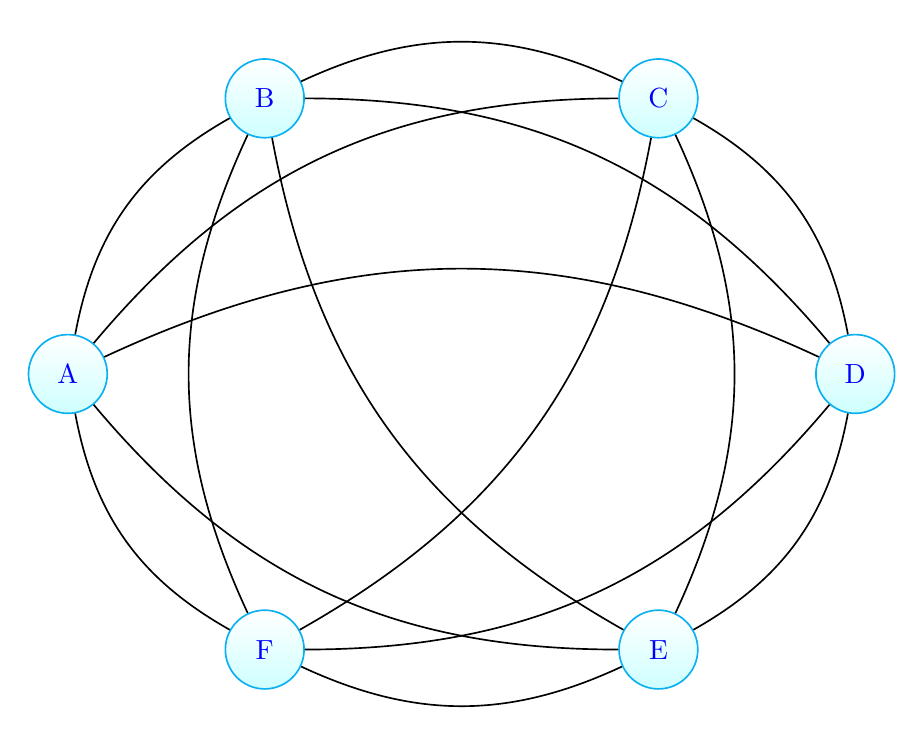
\begin{tikzpicture}[auto, node distance =4 cm and 5cm, on grid , semithick, scale = 1.0,
            state/.style ={ circle ,top color =white , bottom color = processblue!20 ,
            draw,processblue , text=blue , minimum width =1 cm, scale = 1.0}]
        
        %\node [estilo del nodo] (nombre del nodo) [posicion relativa]/at (posicion,absoluta) {};
        
        \node[state] (A) at (-5, 0) {A};
        \node[state] (B) at (-2.5, 3.5) {B};
        \node[state] (C) at (2.5, 3.5) {C};
        \node[state] (D) at (5, 0) {D};
        \node[state] (E) at (2.5, -3.5) {E};
        \node[state] (F) at (-2.5, -3.5) {F};
        
        \path (A) edge [bend right = -25] (B);
        \path (A) edge [bend right = -25] (C);
        \path (A) edge [bend right = -25] (D);
        \path (A) edge [bend right = 25] (E);
        \path (A) edge [bend right = 25] (F);
        
        \path (B) edge [bend right = -25] (C);
        \path (B) edge [bend right = -25] (D);
        \path (B) edge [bend right = 25] (E);
        \path (B) edge [bend right = 25] (F);

        \path (C) edge [bend right = -25] (D);
        \path (C) edge [bend right = -25] (E);
        \path (C) edge [bend right = -25] (F);

        \path (D) edge [bend right = -25] (E);
        \path (D) edge [bend right = -25] (F);

        \path (E) edge [bend right = -25] (F);




        %si queremos un loop
        %\path (A) edge [loop left] node[left] {$1/4$} (A);
    \end{tikzpicture}

    \pagebreak

    b) Supongamos que hay un total de $n$ municipios en una ciudad. Para asociar un grafo a 
    la vecindad entre municiopios, tenemos que definir quienes serán los vértices del grafo. Es 
    conveniente definir a cada municipio como un vértice, entonces el conjunto de vértices 
    estará dado como:
    \begin{equation}
        V = \{ m1, m2, ... , m_n \},
    \end{equation}
    donde el elemento $m_i$ significa el municipio número $i$.\\
    \\Como sólo nos interesa saber qué municipios comparten vecindad, entones el grafo será no 
    orientado y trazaremos aristas entre los vértices bajo la siguiente regla:
    \begin{equation}
        (i, j) \in U \subset V \times V,
    \end{equation}
    sólo si $i$ es vecino de $j$.
%%---------------------------Problema9----------------------------------
%-----------------------------------------------------------------------
\section{Problema}


%%---------------------------Problema10----------------------------------
%-----------------------------------------------------------------------
\section{}
        Un agricultor dispone de un terreno de 5 hectáreasdividido en 4 partes iguales. Se 
        pueden sembrar 4 productos A, B, C, D. Para evitar el empobrecimiento del terreno 
        es necesario rotar cada año el cultivo en cada una de las 4 partes. Al comenzar se 
        debe cultivar cada uno de los productos en una de las 4 partes.

        \begin{table}[h]
            \begin{center}
            
                
            
                \begin{tabular}{|c|c|c|c|c|}
                    \hline
                    \diagbox{Año $n-1$}{Año $n$} & A & B & C & D \\
                    \hline
                                            A   &   & 5 &   & 6 \\
                                                \hline
                                            B   &   &   & 7 &   \\
                                                \hline
                                            C   & 3 &   &   & 9 \\
                                                \hline
                                            D   & 5 & 7 & 4 &   \\
                    \hline
                
                \end{tabular}   
            
            \end{center}
            \caption{}
        \end{table}


        \begin{figure}[h]

 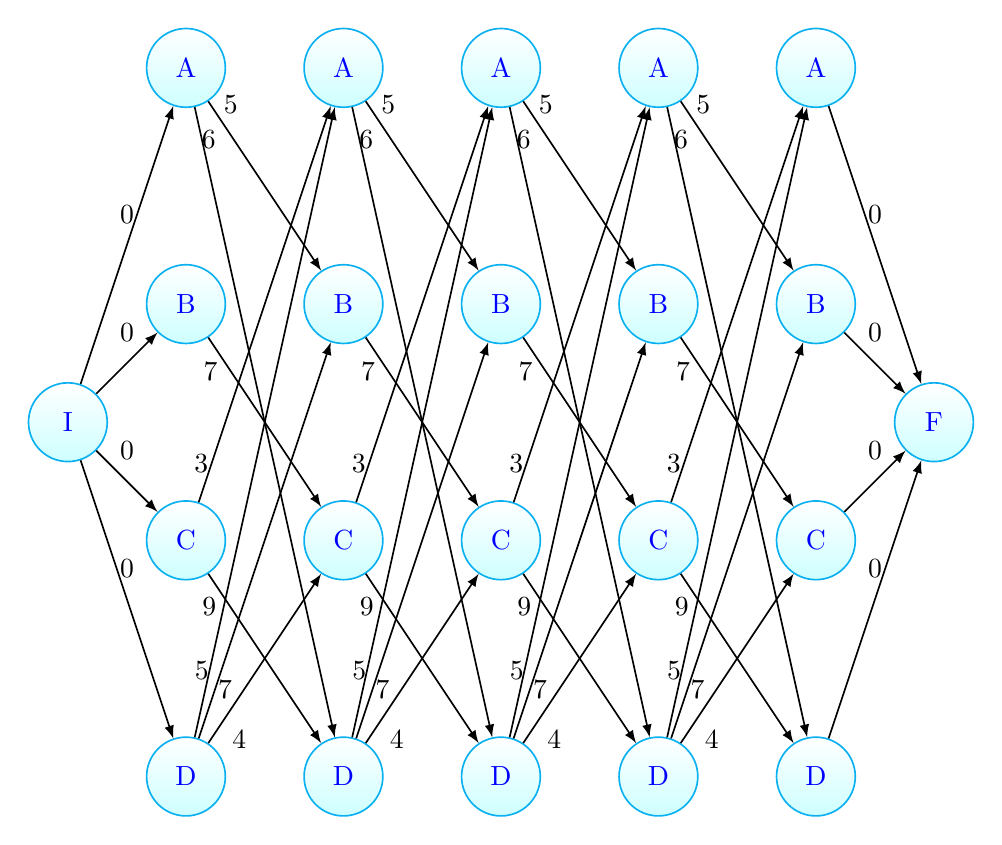
\begin{tikzpicture}[-latex, auto, node distance =4 cm and 5cm, on grid , semithick, scale = 1.0,
            state/.style ={ circle ,top color =white , bottom color = processblue!20 ,
            draw,processblue , text=blue , minimum width =1 cm, scale = 1.0}]
        
        %\node [estilo del nodo] (nombre del nodo) [posicion relativa]/at (posicion,absoluta) {};
        
        \node[state] (I) at (-5, 0) {I};

        \node[state] (A) at (-3.5, 4.5) {A};
        \node[state] (B) at (-3.5, 1.5) {B};
        \node[state] (C) at (-3.5, -1.5) {C};
        \node[state] (D) at (-3.5, -4.5) {D};

        \node[state] (A1) at (-1.5, 4.5) {A};
        \node[state] (B1) at (-1.5, 1.5) {B};
        \node[state] (C1) at (-1.5, -1.5) {C};
        \node[state] (D1) at (-1.5, -4.5) {D};

        \node[state] (A2) at (0.5, 4.5) {A};
        \node[state] (B2) at (0.5, 1.5) {B};
        \node[state] (C2) at (0.5, -1.5) {C};
        \node[state] (D2) at (0.5, -4.5) {D};

        \node[state] (A3) at (2.5, 4.5) {A};
        \node[state] (B3) at (2.5, 1.5) {B};
        \node[state] (C3) at (2.5, -1.5) {C};
        \node[state] (D3) at (2.5, -4.5) {D};

        \node[state] (A4) at (4.5, 4.5) {A};
        \node[state] (B4) at (4.5, 1.5) {B};
        \node[state] (C4) at (4.5, -1.5) {C};
        \node[state] (D4) at (4.5, -4.5) {D};

        \node[state] (F) at (6, 0) {F};

        %%--------------------------caminos---_-------------
        
        \path (I) edge node[above = 0.15 cm] {$0$} (A);
        \path (I) edge node[above = 0.15 cm] {$0$} (B);
        \path (I) edge node[above = 0.15 cm] {$0$} (C);
        \path (I) edge node[above = 0.15 cm] {$0$} (D);
        
        \path (A) edge node[above = 0.15 cm, pos = 0.20] {$5$} (B1);
        \path (A) edge node[above = 0.15 cm, pos = 0.10] {$6$} (D1);
        \path (B) edge node[below = 0.15 cm, pos = 0.02] {$7$} (C1);
        \path (C) edge node[above = 0.15 cm, pos = 0.02] {$3$} (A1);
        \path (C) edge node[below = 0.15 cm, pos = 0.01] {$9$} (D1);
        \path (D) edge node[above = 0.20 cm, pos = 0.05] {$5$} (A1);
        \path (D) edge node[below = 0.15 cm, pos = 0.20] {$7$} (B1);
        \path (D) edge node[right = 0.15 cm, pos = 0.02] {$4$} (C1);

        \path (A1) edge node[above = 0.15 cm, pos = 0.20] {$5$} (B2);
        \path (A1) edge node[above = 0.15 cm, pos = 0.10] {$6$} (D2);
        \path (B1) edge node[below = 0.15 cm, pos = 0.02] {$7$} (C2);
        \path (C1) edge node[above = 0.15 cm, pos = 0.02] {$3$} (A2);
        \path (C1) edge node[below = 0.15 cm, pos = 0.01] {$9$} (D2);
        \path (D1) edge node[above = 0.20 cm, pos = 0.05] {$5$} (A2);
        \path (D1) edge node[below = 0.15 cm, pos = 0.20] {$7$} (B2);
        \path (D1) edge node[right = 0.15 cm, pos = 0.02] {$4$} (C2);

        \path (A2) edge node[above = 0.15 cm, pos = 0.20] {$5$} (B3);
        \path (A2) edge node[above = 0.15 cm, pos = 0.10] {$6$} (D3);
        \path (B2) edge node[below = 0.15 cm, pos = 0.02] {$7$} (C3);
        \path (C2) edge node[above = 0.15 cm, pos = 0.02] {$3$} (A3);
        \path (C2) edge node[below = 0.15 cm, pos = 0.01] {$9$} (D3);
        \path (D2) edge node[above = 0.20 cm, pos = 0.05] {$5$} (A3);
        \path (D2) edge node[below = 0.15 cm, pos = 0.20] {$7$} (B3);
        \path (D2) edge node[right = 0.15 cm, pos = 0.02] {$4$} (C3);

        \path (A3) edge node[above = 0.15 cm, pos = 0.20] {$5$} (B4);
        \path (A3) edge node[above = 0.15 cm, pos = 0.10] {$6$} (D4);
        \path (B3) edge node[below = 0.15 cm, pos = 0.02] {$7$} (C4);
        \path (C3) edge node[above = 0.15 cm, pos = 0.02] {$3$} (A4);
        \path (C3) edge node[below = 0.15 cm, pos = 0.01] {$9$} (D4);
        \path (D3) edge node[above = 0.20 cm, pos = 0.05] {$5$} (A4);
        \path (D3) edge node[below = 0.15 cm, pos = 0.20] {$7$} (B4);
        \path (D3) edge node[right = 0.15 cm, pos = 0.02] {$4$} (C4);

        \path (A4) edge node[above = 0.15 cm] {$0$} (F);
        \path (B4) edge node[above = 0.15 cm] {$0$} (F);
        \path (C4) edge node[above = 0.15 cm] {$0$} (F);
        \path (D4) edge node[above = 0.15 cm] {$0$} (F);
        



        %si queremos un loop
        %\path (A) edge [loop left] node[left] {$1/4$} (A);
        
        %otras opciones: 
        %\path (A) 
        %    edge [left] node [blue, pos=0.5, sloped, above] {$0 \rightarrow [x = x.0.0]$} (B)
        %    edge [left] node [cyan, pos=0.8]{$1 \rightarrow [x = x.0.1]$} (C)(B) 
        %    edge [loop above] node [align=center] {$0 \rightarrow$ \\ $[x = x.0]$ }   (B)
        %    edge [bend right,left] node  {$1 \rightarrow [x = x.1]$ }   (C)
        %    edge [] node [red, pos=0.2] {$\$  \rightarrow  [x = x.0.\$]$ } (D);  


    \end{tikzpicture}
     \caption{}
\end{figure}  

        \pagebreak
%%---------------------------Problema11----------------------------------
%------------------------------------------------------------------------
\section{Problema}
        Construya los grafos asociados a un proyecto cuyas actividades y antecedentes se dan a 
        continuación:
        \begin{table}[h]
            \begin{center}
            
                
            
                \begin{tabular}{|c|c|}
                    \hline
                    Actividades & Antecedentes \\
                    \hline
                    1 -2 & -- \\
                    \hline
                    1 -3 & -- \\
                    \hline
                    1 -4 & -- \\
                    \hline
                    1 -5 & -- \\
                    \hline
                    2 -4 & 1 -2 \\
                    \hline
                    3 -4 & 1 -3 \\
                    \hline 
                    4 -5 & 2 -4, 1 -4, 3 -4 \\
                    \hline 
                    5 -6 & 4 -5, 1 -5 \\
                    \hline
                    6 -7 & 6 -6                    \\
                    \hline                      
                
                \end{tabular}   
            
            \end{center}
            \caption{}
        \end{table}

        El grafo asociado es:

        \begin{figure}[h]


    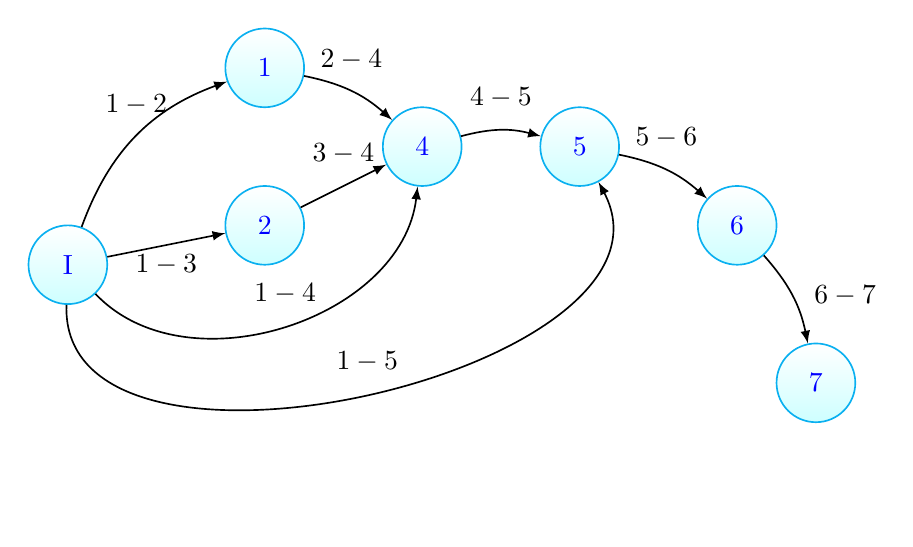
\begin{tikzpicture}[-latex, auto, node distance =4 cm and 5cm, on grid , semithick, scale = 1.0,
            state/.style ={ circle ,top color =white , bottom color = processblue!20 ,
            draw,processblue , text=blue , minimum width =1 cm, scale = 1.0}]
        
            %\node [estilo del nodo] (nombre del nodo) [posicion relativa]/at (posicion,absoluta) {};
            \node[state] (I) at (0, 0) {I};
            \node[state] (n1) at (2.5, 2.5) {1};
            \node[state] (n2) at (2.5, 0.5) {2};
            
            \node[state] (n4) at (4.5, 1.5) {4};
            \node[state] (n5) at (6.5, 1.5) {5};
            \node[state] (n6) at (8.5, 0.5) {6};
            \node[state] (n7) at (9.5, -1.5) {7};
        
    
            \path (I) edge [bend right = -25] node[above = 0.15 cm] {$1 -2$} (n1);
            \path (I) edge node[below = 0.0 cm] {$1 -3$} (n2);
            \path (I) edge [bend right = 65] node[above = 0.15 cm] {$1 -4$} (n4);
            \path (I) edge [bend right = 105] node[above = 0.15 cm] {$1 -5$} (n5);

            \path (n1) edge [bend right = -15] node[above = 0.15 cm] {$2 -4$} (n4);
            \path (n2) edge node[above = 0.15 cm] {$3 -4$} (n4);

            \path (n4) edge [bend right = -15] node[above = 0.15 cm] {$4 -5$} (n5);
            \path (n5) edge [bend right = -15] node[above = 0.15 cm] {$5 -6$} (n6);
            \path (n6) edge [bend right = -15] node[right = 0.15 cm] {$6 -7$} (n7);
    
    
            %si queremos un loop
            %\path (A) edge [loop left] node[left] {$1/4$} (A);
        \end{tikzpicture}
        
        \caption{}
    \end{figure}

%%---------------------------Otros problemas----------------------------------
%-----------------------------------------------------------------------
\section{Problema que resolvimos en clase as}
   



%---------------------------
\end{document}
%---------------------------

